\section{Neuron}

\subsection{Cell}

\begin{figure}[!h]
    \centering
    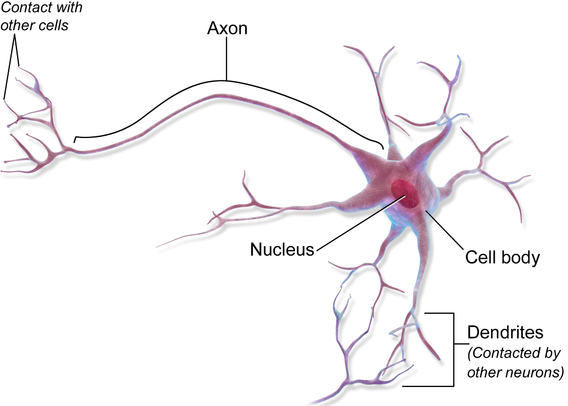
\includegraphics[scale=1]{Media/MultipolarNeuron.png}
    \caption[Multipolar neuron cell]{Multipolar neuron cell \textit{(sizes and shapes vary)}}
    \label{fig:MultipolarNeuronCell}
\end{figure}

Without going into a details. There exist a few type of neural cell. In our mathematical model we use \textit{Multipolar neural cell} which is shown on \hyperref[fig:MultipolarNeuron]{Figure \ref{fig:MultipolarNeuron}}. This one constitute the majority of neurons in the brain and include motor neurons and interneurons.

The way it works is such that it gather input signals through \textit{dendrites} and produce one output signal through \textit{axon}. The input signals are sum by \textit{nucleus} and only if specific value is obtains the \textit{axon} is activated. Both input and output signal are also modified while they are transmitted to \textit{nucleus} or next cell. Modification depends on \textit{nucleus} and thickness of \textit{neurolemma (which is not shown on the figure)}. This signal changing part is a place where the \textit{neurons network} knowledge is contained.

\newpage
\subsection{Model}

\begin{figure}[!h]
    \centering
    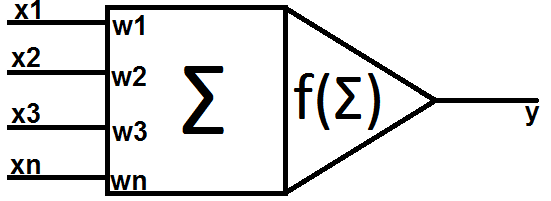
\includegraphics[scale=0.5]{Media/Neuron.png}
    \caption{Basic neuron/perceptron model}
    \label{fig:NeuronModel}
\end{figure}

Such \textit{multipolar neuron cell} mechanism can be easily model. Each \textit{neuron} input is represented by $x_n$ and multiply by corresponding factors $w_n$ which represents change in \textit{neuron} input signal. All signals are sum (that represents \textit{nucleus} function) and then processed by the \textit{activation function} (which is representation of the active or inactive \textit{axon} and also serves other purposes - more about that later in this chapter).
$$f\left(\sum\limits_{i=1}^n x_iw_i\right) = y$$